\begin{questions}


\question{
    We implement a distributed memory
    (i.e., MPI) parallel version of the two-dimensional Jacobi smoother from the second assignment. 
    This is an extension of the one-dimensional case available in the class repository.
    We will use a uniform domain splitting and exchange unknowns
    corresponding to neighboring points (the so-called ghost points) on different processors.
    To make our lives easier, we only consider uniform splittings of all unknowns using $p = 4^j$,
    $j = 0, 1, 2, 3,\dots$ processors. Additionally we assume that we deal with $N = 2^jN_l$ unknowns
    in the $x$ and $y$ directions, such that each processor works on $N_l^2$ unknowns.
    
    Run your implementation on Prince. For large $N_l$ (e.g., $N_l = 100$), perform a weak scaling
    study and plot the timings (fix the number of iterations for this study) as you increase
    the number of points and MPI tasks. Then choose $N_l$ as large as possible to fit on one
    processor, and perform a strong scaling study, i.e., keep the problem size unchanged while
    increasing the number of MPI task, and plot the speedup compared to the ideal speedup.
}

\begin{solution}
    Our implementation is in the file \texttt{jacobi2D-mpi.cpp}, We will discuss our 
    notable considerations when implementing the algorithm. On one process, we
    order the expanded local unknowns in a column major order, illustrated in 
    Figure \ref{fig:local} below
    for $N_l = 2$.
    \begin{center}
        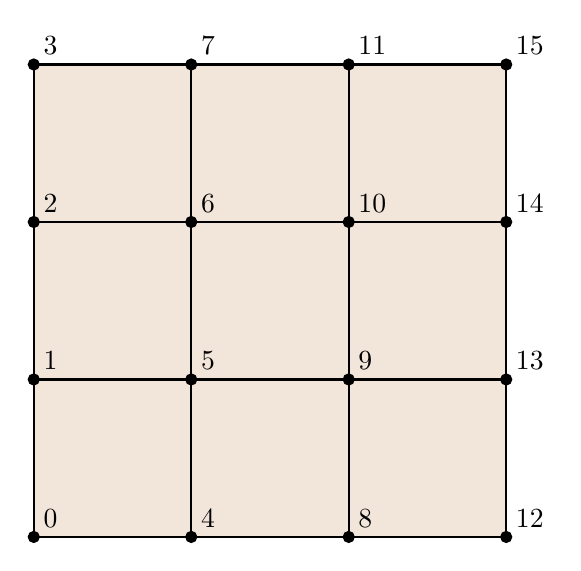
\begin{tikzpicture}
          \foreach \x in {0,2,4}{
            \foreach \y in {0,2,4}{
            %   \filldraw[draw=black,thick,fill=brown!20!white] (\x,\y) rectangle ++(2,2);
            %   \draw[draw=black,thick] (\x+2,\y) -- (\x,\y+2);
              \draw[draw=black,thick,fill=brown!20!white] (\x+6,\y) rectangle ++(2,2);
            }
          }
          \filldraw[black] (6,0) circle (2pt)  node[above right] {0};
          \filldraw[black] (6,2) circle (2pt)  node[above right] {1};
          \filldraw[black] (6,4) circle (2pt)  node[above right] {2};
          \filldraw[black] (6,6) circle (2pt)  node[above right] {3};
          \filldraw[black] (8,0) circle (2pt)  node[above right] {4};
          \filldraw[black] (8,2) circle (2pt)  node[above right] {5};
          \filldraw[black] (8,4) circle (2pt)  node[above right] {6};
          \filldraw[black] (8,6) circle (2pt)  node[above right] {7};
          \filldraw[black] (10,0) circle (2pt)  node[above right] {8};
          \filldraw[black] (10,2) circle (2pt)  node[above right] {9};
          \filldraw[black] (10,4) circle (2pt)  node[above right] {10};
          \filldraw[black] (10,6) circle (2pt)  node[above right] {11};
          \filldraw[black] (12,0) circle (2pt)  node[above right] {12};
          \filldraw[black] (12,2) circle (2pt)  node[above right] {13};
          \filldraw[black] (12,4) circle (2pt)  node[above right] {14};
          \filldraw[black] (12,6) circle (2pt)  node[above right] {15};
        \end{tikzpicture}
        \captionof{figure}{Local unknown ordering for $N_l = 2$. Grid is $(N_l+2)\times(N_l+2)$
        to store ghost points.}
        \label{fig:local}
    \end{center}
    
    In this configuration, the key values are the ``internal" unknowns 5, 6, 9, and 10,
    and it will receive the points necessary for the five-point stencil---1, 
    2, 4, 8, 7, 11, 13, and 14---with its neighbors if it is not on the edge of the domain. 
    It will send its corresponding ``edge unknowns" (in this case also 5, 6, 9, and 10)
    to its neighbors for their update step. The  ``corner" unknowns 0, 3, 12, and 15
    are stored for convenience, but they are never used to update the solution or to
    compute the residual.
    
    We assume the processes take each uniform section of the unknowns as described
    in the assignment, e.g., for $j=1$ as in Figure \ref{fig:processes}.
    \begin{center}
        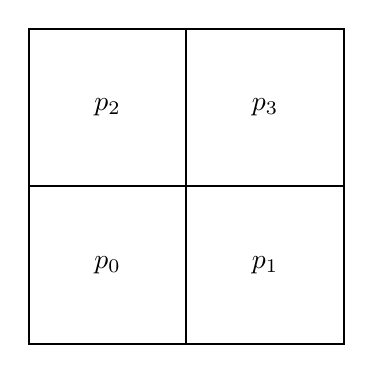
\begin{tikzpicture}
          \foreach \x in {0,2}{
            \foreach \y in {0,2}{
            %   \filldraw[draw=black,thick,fill=brown!20!white] (\x,\y) rectangle ++(2,2);
            %   \draw[draw=black,thick] (\x+2,\y) -- (\x,\y+2);
              \draw[draw=black,thick] (\x+6,\y) rectangle ++(2,2);
            }
          }
          \filldraw[black] (6+1,0+1) node {$p_0$};
          \filldraw[black] (6+1,2+1) node {$p_2$};
          \filldraw[black] (8+1,0+1) node {$p_1$};
          \filldraw[black] (8+1,2+1) node {$p_3$};
        \end{tikzpicture}
        \captionof{figure}{Partitioning of the domain for different MPI processes, ($j=1$)}
        \label{fig:processes}
    \end{center}
    
    Communicating points left and right (unknowns 1, 2, 5, 6, 9, 10, 13, and 14)
    is straightforward since each edge is stored sequentially in memory. For the top
    and bottom edges (unknowns 4--11), this is not the case (The correct ordering to keep
    in mind is $\{4,8\}$, \{5,9\}, etc.). So to communicate with neighboring processes,
    we must first store the memory sequentially by copying the values into a temporary
    address, both for sending and receiving messages. This is the purpose of the
    variables \texttt{tmpout}, \texttt{tmpin}, \texttt{tmp2out}, and \texttt{tmp2in}. 
    
    Our results for the weak and strong scaling tests are summarized in the tables and
    figure below. For the weak scaling test, we run the Jacobi method for 1,000 iterations
    for each of the parameter combinations in Table \ref{tab:weak_jacobi}.
    Ideally, for weak scaling the runtime would be constant for all four of these
    instances, but this is not the case. We expect the reasonable slowdown that occurs
    from $j=0$ to $j=1$ and $j=3$, but the timing for $j=2$ is an outlier. This is
    possibly because the Prince scheduler assigned each of these jobs to different
    nodes, and hence different architectures. The $j=2$ partition, c42-02 may just
    perform more slowly for these flop-intensive jobs.
    
    \begin{minipage}{0.48\textwidth}
    \begin{center}
        \begin{tabular}{|c|c|c|c|r|}
        \hline
        $j$ & $N_l$ & $N$ & $p$ & Time (s) \\
        \hline\hline
        0 & 100 & 100 & 1 & 0.0217 \\ 
        \hline
        1 & 100 & 200 & 4 & 8.7512 \\ 
        \hline
        2 & 100 & 400 & 16 & 203.1598 \\ 
        \hline
        3 & 100 & 800 & 64 & 86.4756 \\ 
        \hline
        \end{tabular}
        \captionof{table}{Weak scaling test for MPI Jacobi}
        \label{tab:weak_jacobi}
    \end{center}
    \end{minipage}
    \begin{minipage}{0.48\textwidth}
    \begin{center}
        \includegraphics[width=0.85\textwidth]{Images/jacobi_weak_plot.jpg}
        \captionof{figure}{Weak scaling run times}
        \label{fig:weak_plot}
    \end{center}
    \end{minipage}
    
    For our strong scaling test, we set $N$ to be a constant and decreased the 
    number of Jacobi iterations to 100. Then, we increased $N$ until all four
    jobs could complete in under one hour of computation time with 10GB of
    memory allocated. The largest $N$ that satisfies this criterion is 
    approximately 800. However, as Figure \ref{fig:strong_plot} illustrates,
    this $N$ is too small to overcome the MPI communication overhead, and we
    observe slowdown for large number of processes. We are currently testing
    jobs which allow for more computation time so that we can see a more
    accurate asymptotic strong scaling rate, and we will update this document
    when those jobs complete.
    
    \begin{minipage}{0.46\textwidth}
    \begin{center}
        \begin{tabular}{|c|c|c|c|r|}
        \hline
        $j$ & $N_l$ & $N$ & $p$ & Time (s) \\
        \hline\hline
        0 & 800 & 800 & 1 & 1.299 \\ 
        \hline
        1 & 400 & 800 & 4 & 0.487 \\ 
        \hline
        2 & 200 & 800 & 16 & 8.352 \\ 
        \hline
        3 & 100 & 800 & 64 & 8.775 \\ 
        \hline
        \end{tabular}
        \captionof{table}{Strong scaling test for MPI Jacobi}
        \label{tab:strong_jacobi}
    \end{center}
    \end{minipage}
    \begin{minipage}{0.48\textwidth}
    \begin{center}
        \includegraphics[width=0.85\textwidth]{Images/jacobi_strong_plot.jpg}
        \captionof{figure}{Strong scaling run times}
        \label{fig:strong_plot}
    \end{center}
    \end{minipage}
\end{solution}






\question{
    Each of $P$ processors creates an $N$-vector of random numbers.
    The target is to sort the union of all these distributed vectors; this union, let's call it $v$,
    consists of $PN$ numbers and is assumed to be too large to fit into the memory of a single
    processor---thus, a serial sort algorithm cannot be used. The goal is to sort $v$ such that
    every processor roughly holds about $N$ sorted numbers, say $v_i$, and that all elements on
    the processor with rank $i$ are smaller than those on the processor with rank $i + 1$ (for all $i = 0, 1, \dots P-2$). The above repository contains a stub called \texttt{ssort.cpp}. This file
    also contains an outline of the algorithm, which we also discussed in class. The main steps of sample sort are:
    \begin{itemize}
        \item Select local samples
        \item Distribute to buckets
        \item Local sort
    \end{itemize}
    
    Include the MPI rank in the filename (see the example \texttt{file-io.cpp} example file). Run
your implementation of the sorting algorithm on at least 64 cores of Prince, and present
timings (not including the time to initialize the input array or the time to write output to file) depending on the number of elements $N$ to be sorted per processor (report results for
$N = 10^4$, $10^5$, and $10^6$).
}

\begin{solution}
    Our implementation is in the modified file \texttt{ssort.cpp}. The implementation
    is mostly straightforward, although the trickiest part was determining how to
    distribute the integers to each process (i.e., bucket). In the MPI framework,
    this requires counting the number each process $i$ must send to each other process $j$,
    and how many $i$ will receive from $j$. This took some handwork to confirm that
    the memory was treated correctly.
    
    Timings for the listed cases are in Table \ref{tab:sort} below. For $N=10^4$
    and $N=10^5$, the timings are roughly the same since this is likely still the 
    pre-asymptotic regime where the MPI communication dominates run time.
    For $N=10^6$ however, we see the run time increase as the memory load becomes
    significant. Because we assume that the full vector cannot fit on one
    process, we cannot compare the run time to a serial implementation. However, 
    the scaling of a $4\times$ increase in runtime from $N=10^5$ to $N=10^6$ gives
    a rough idea of how the algorithm scales for larger memory requirements.
 	\begin{center}
        \begin{tabular}{|c|c|r|}
        \hline
        $p$ & $N$ & Time(s) \\
        \hline\hline
        $64$ & $10^4$ & 0.072263 \\ 
        \hline
        $64$ & $10^5$ & 0.086920 \\ 
        \hline
        $64$ & $10^6$ & 0.230437 \\ 
        \hline
        \end{tabular}
        \captionof{table}{Sort timings for increasing lengths of local arrays}
        \label{tab:sort}
    \end{center}
\end{solution}


\end{questions}